% Chapter Template

\chapter{Project Plan} % Main chapter title

\label{Chapter2} % Change X to a consecutive number; for referencing this chapter elsewhere, use \ref{ChapterX}

\lhead{Chapter 2. \emph{Project Plan}} % Change X to a consecutive number; this is for the header on each page - perhaps a shortened title

%----------------------------------------------------------------------------------------

\section{Schedule}

The schedule was designed as a Gantt chart, in order to highlight key points in the project and ensure that they were completed on time and according to the set deadlines. This schedule is subject to change as the project progresses, as many unforeseen issues may arise. I have tried to estimate tasks based on difficulty, assigning more time to key points where it is likely that problems will occur (such as the implementation phase). 

\begin{sidewaysfigure}[htbp]
	\centering
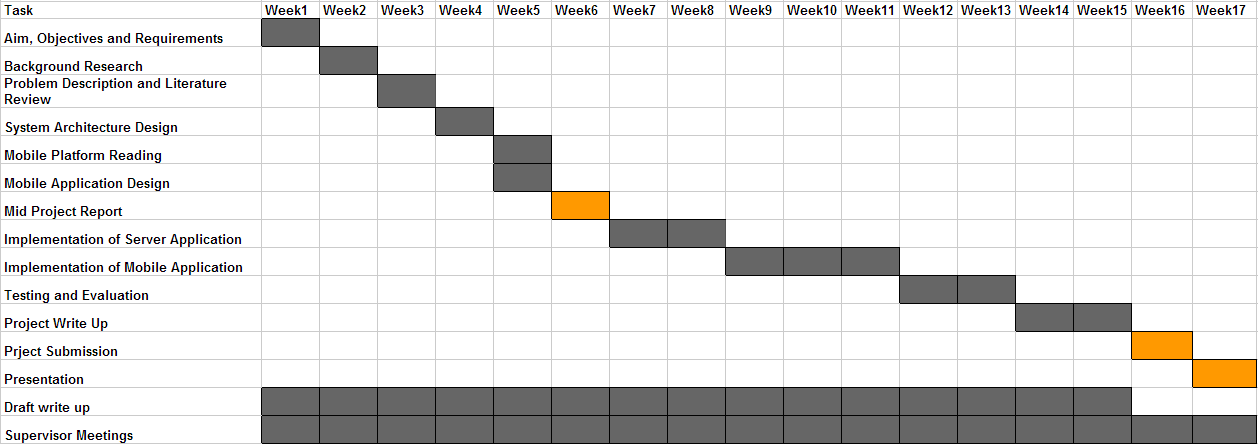
\includegraphics[width=\textheight, keepaspectratio]{Figures/projectgant.png}
		\rule{35em}{0.5pt}
	\caption[Gantt Chart showing the schedule of the project]{Gantt Chart showing the schedule of the project}
	\label{fig:projectgant}
\end{sidewaysfigure}

A table was also created to compare objectives with deliverable deadlines.

\begin{figure}[htbp]
	\centering
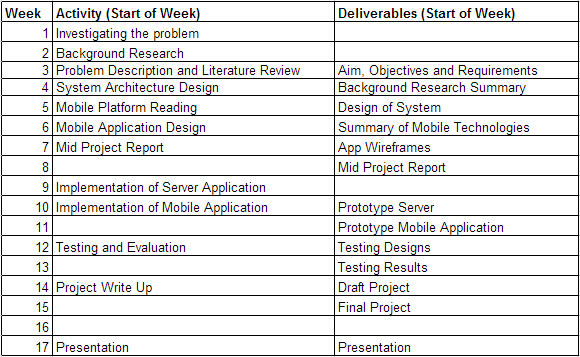
\includegraphics[width=\textwidth,height=\textheight,keepaspectratio]{Figures/projectplan.png}
		\rule{35em}{0.5pt}
	\caption[Table showing the schedule of the project]{Table showing the schedule of the project}
	\label{fig:projectplan}
\end{figure}

The project has been split four main components, consisting of research, design, implementation and evaluation. These areas are then sub-divided into appropriate sections, targeting individual parts of the system, individual objectives and individual deliverables.

The following sections will explain these components, what parts of the project they will address and how they will be executed successfully.

%----------------------------------------------------------------------------------------

\section{Background Research}

The research component will aim to get a better understanding of the problem, how I can address my aims and objectives and highlighting the current research in the field. This research will aid my own project by highlighting areas that need to be addressed, outlining unforeseen problems and finding technologies that I might be useful to my implementation.

%----------------------------------------------------------------------------------------

\section{Design}

The design component will aim to design the entire system, addressing all objectives whilst making the system both flexible and scalable.

\subsection{Methodologies}

I will choose a software engineering methodology that best fits the development style of the project, explaining how it works and how it is executed successfully. I will also identify the programming languages I will be using, any programming patterns that are useful in the design of the system and Technologies I will use.

\subsection{Flexibility}

Although the system is a prototype, I aim to create it such that it can be adapted in the future. The system will therefore be designed in a way such that additional platforms can be added easily. The system should also be designed in a way that it is feature independent, eliminating dependencies in the code. This will allow more features to be added easily in the future.

\subsection{Scalability}

The system will also be designed to be scalable. It must be able to scale with user demand, be fault tolerant and and appear seamless to the end user, allowing for a smooth service at all times. I will talk about the various problems involved and how I will design the system to overcome them.

\subsection{Problems}

Many problems must be overcome in the implementation phase, such as data security, synchronising data and many more. These problems must be planned in advance, and so I will discuss in detail the problems that the system faces and my proposed solutions to them.

%----------------------------------------------------------------------------------------

\section{Implementation}

The implementation of the system will occur in two separate platforms, the client and the server. These will sometimes overlap as some code will be shared between them, however for the most part, I will discuss issues unique to each platform separately.

For the server platform, I will discuss how I implemented the communication and data storage features and the overall structure of the server system.

For the client platform, I will discuss how the user interface is created, how it communicates with the server and any issues that I encountered.

%----------------------------------------------------------------------------------------

\section{Evaluation}

The evaluation component will show how well my prototype system does in solving my aims and objectives identified in the project. I will analyse the results of user evaluation methods to evaluate the prototype, discussing the results and identifying key parts of my solution that need to be improved. I plan to evaluate on the following questions:

\begin{itemize}
	\item How easy to use is the mobile application?
	\item Does the solution work? Does it fail occasionally?
	\item Is the solution missing key features?
	\item Would patients find the mobile application useful?
	\item Does the solution reduce wasted appointments?
	\item Does the solution reduce staff resources required for managing appointments?
	\item Does the solution increase the user experience when managing appointments?
\end{itemize}

\section{Conclusion}

From this evaluation, I will formulate a conclusion, reviewing my design choices, how accurate my expectations were and discussing future extensions that this project could inspire.

%----------------------------------------------------------------------------------------
